\chapter[Draft of the application]{Draft of the application}
\label{draft}
Within this thesis, we will develop an application (with focus on the backend system) to handle all these problems that have been described above within the section about the current situation. This master thesis will handle the planning respectively cost estimation of the different parts/features of the general system and will, after the needed technologies respectively frameworks are elaborated and evaluated, include a prototypical implementation of the needed components of the backend system. 

But at first, we will start with the first step within each development process; the requirements engineering.

\section{Requirements engineering}
First of all, a requirement is defined as "[...]A condition or capability that must be met or possessed by a system or system component to satisfy a contract, standard, specification, or other formally imposed documents[...]" (\cite{IEEEReq}).

We started the development of the application with a requirements engineering meeting together with our \textit{customer}. Within this meeting, we talked about the main ideas of the application and tried to grasp the needed functionality. In the end, we ended up with a couple of cards with written user stories. Some of these cards are shown in Figure \ref{cards}.

\begin{figure}[th]
\centerline{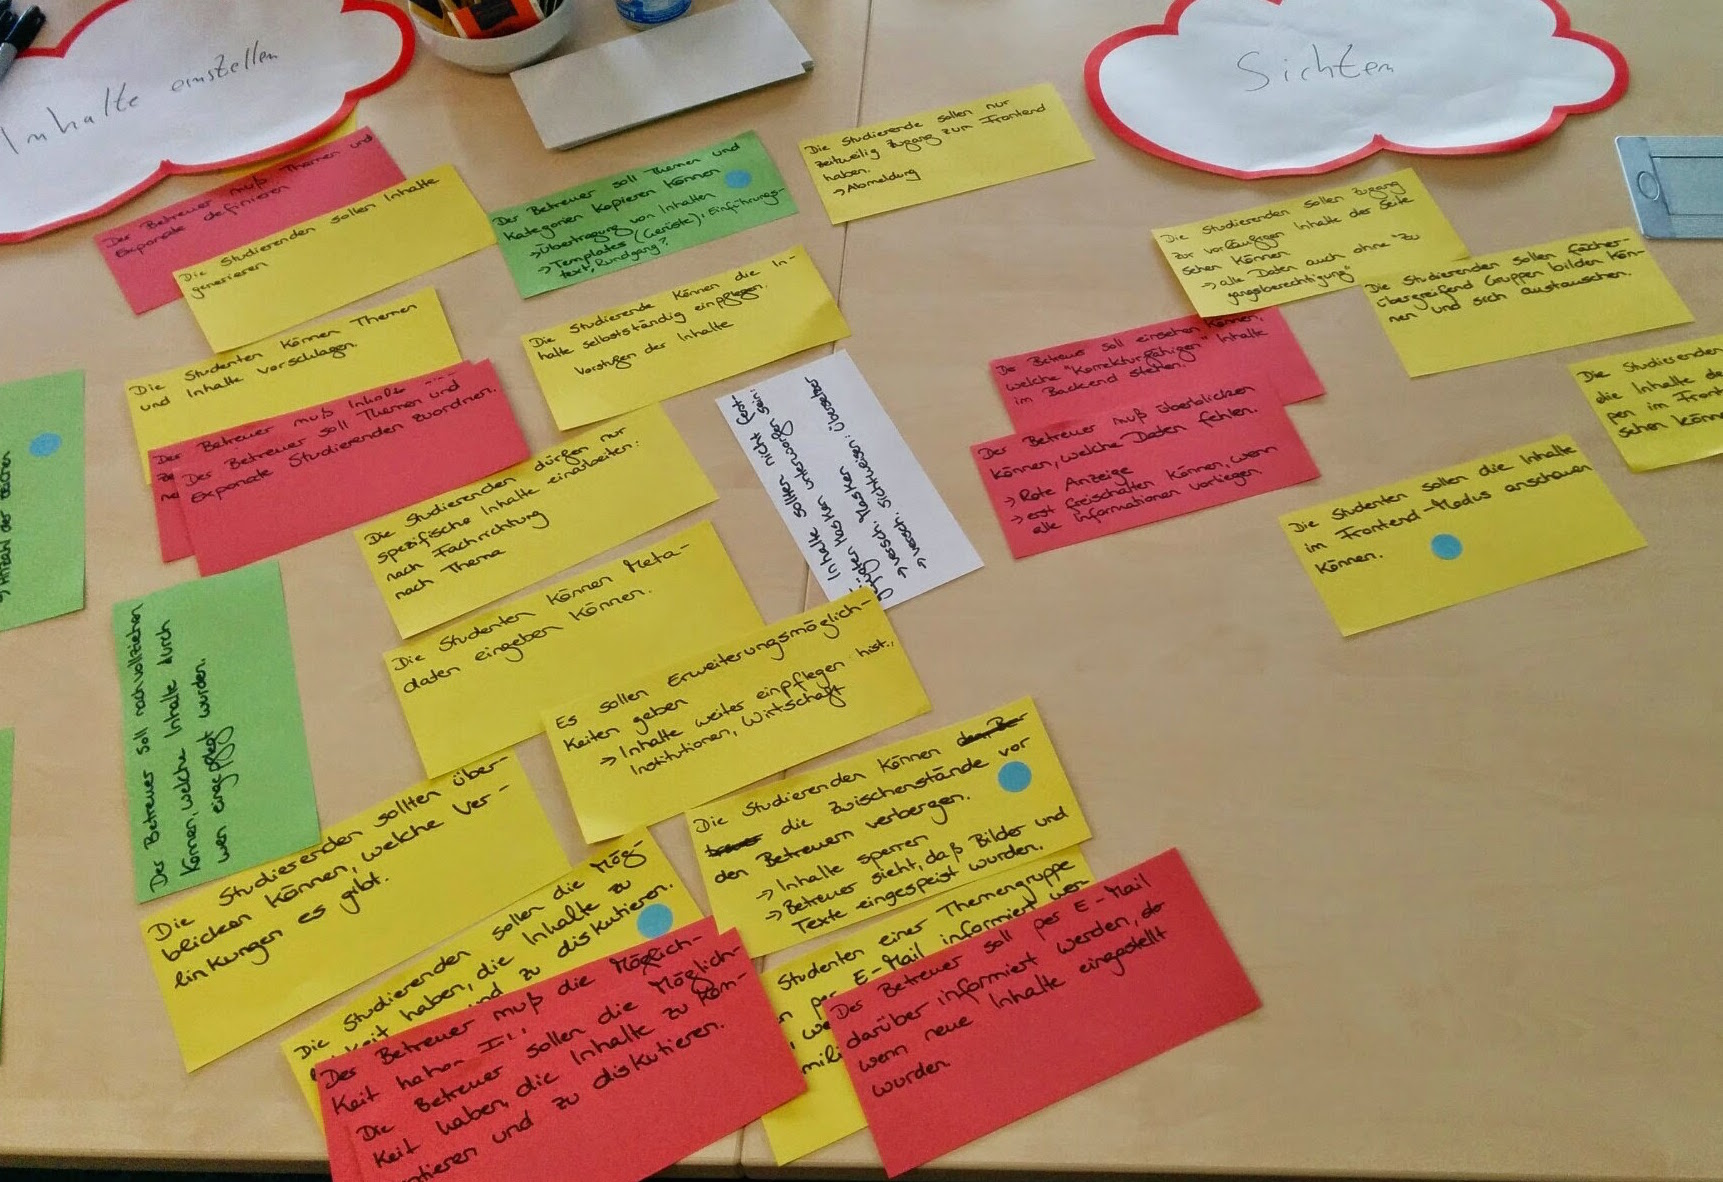
\includegraphics[width=1\textwidth]{gfx/cards.jpg}}
\caption{Some of the requirement cards that has been sorted within the requirements engineering meeting.}
\label{cards}
\end{figure} 

After this meeting, these stories got refined to concrete high level requirements, which are measurable and prioritized. A complete list of all requirements, which were derived from these user stories, can be found within the appendix in tables \ref{RequirementsBackendSupervisor}, \ref{RequirementsBackendStudent}, \ref{RequirementsBackendMaster}, \ref{RequirementsBackendMisc} and \ref{RequirementsFrontend}. These requirements can directly be used to derive some the needed test cases for the \ac{TDD} approach.

One of these main features that has been elaborated in this meeting, was the need for four different roles within the complete system. We will now take a more detailed look at these roles within the following section.

\section{Use Cases}
The system on its whole will have four different kinds of users, which correspond to four different roles within the system. The roles are briefly described in the following:

\begin{enumerate}
	\item Supervisors: Supervisors work at the university and create groups, topics and are able to review the information of their groups. The main goal of a supervisor is the supervision of groups.
	\item Students: Students are placed in groups by their supervisor and work on a specific topic. They are able to hand in their work for review by the supervisor. 
	\item Admin: The admins are able to assign users to specific roles and edit the system itself (e.g., edit translations, etc.).
	\item Master: People, who have the role \textit{Master}, are able to accept respectively reject topics for the front-end application
\end{enumerate}

These four different roles are also shown in Figure \ref{usecase} as an \ac{UML2} use case diagram, which is placed in the appendix. Figure shows the roles together with the functionality that gets invoked by these roles. 	

After we have now seen the different roles that are involved in this system, we will include two use case tables as an example for the usage of the system here. However, a complete list of use case scenarios would be to large for this thesis.

 \begin{table}[h]
\scriptsize
 \caption{Use Case Scenario: Student changes content of a topic}
 \begin{tabular}{lll}
	\toprule
  Step: & Involved: & Description of the activity: \\ 
\cmidrule(rl){1-1}\cmidrule(rl){2-2}\cmidrule(rl){3-3}
  	0 	& Student & logs into the system \\
	1	& Student & navigates to the correct group \\
	2	& Student & navigates to the topic he wants to work on \\
	3	& Student & changes content on the topic \\
	4	& Student & saves the changes \\	
	5	& Student & logs out \\
	\bottomrule
 \end{tabular}
 \label{tab:ucTopicChange}
 \end{table} 

Table \ref{tab:ucTopicChange} shows that when a student wants to change the content of a topic he is working on, he needs to log into the system, navigate to the group and topic and is then able to change the content.
 
 \begin{table}[h]
\scriptsize
 \caption{Use Case Scenario: Supervisor creates a new group}
 \begin{tabular}{lll}
	\toprule
  Step: & Involved: & Description of the activity: \\ 
\cmidrule(rl){1-1}\cmidrule(rl){2-2}\cmidrule(rl){3-3}
  	0 	& Supervisor & logs into the system \\
	1	& Supervisor & navigates to create group view \\
	2	& Supervisor & inputs name, member, topics, etc. \\
	3	& Supervisor & saves the group \\	
	4	& Supervisor & logs out \\
	\bottomrule
 \end{tabular}
 \label{tab:ucGroupCreation}
 \end{table} 

The second use case scenario is shown within Table \ref{tab:ucGroupCreation}. It shows that it will be quite easy for a supervisor to create a new group. The only steps he needs to take is to log into the system, open the correct view and input all needed information (e.g., members of the group). 

\todo{include simple sequence diagrams}

Now, after we have seen what the application is about, we will now take a closer look at the planned architecture.

\section{Architecture of the application}
\label{architecture}
The architecture design within agile projects is slightly different from the design in common respectively classical development projects. Within a classical development process, one would design the architecture of the system on its whole, before the actual programming phase is started (\cite{Patterns:2009aa}). This is, obviously, not applicable within an agile development approach. As \cite{Mast2013} points out, agile architecture design has the following important attributes:

\begin{enumerate}
	\item At the beginning, one has only an idea about the architecture, which describes the most important constraints. However, there has to be enough space to be able to adapt the architecture to new or changing requirements within the development process.
	\item This enables the developer to be able to use an iterative development style and to postpone important development choices to the \textit{Least Responsible Moment}. The \textit{Least Responsible Moment} is the latest possible point in time, where you can implement an architecture decision.
	\item This way, detailed structures and technical concepts are created on-the-fly, while the application gets developed.
\end{enumerate}

\begin{figure}[th]
\centerline{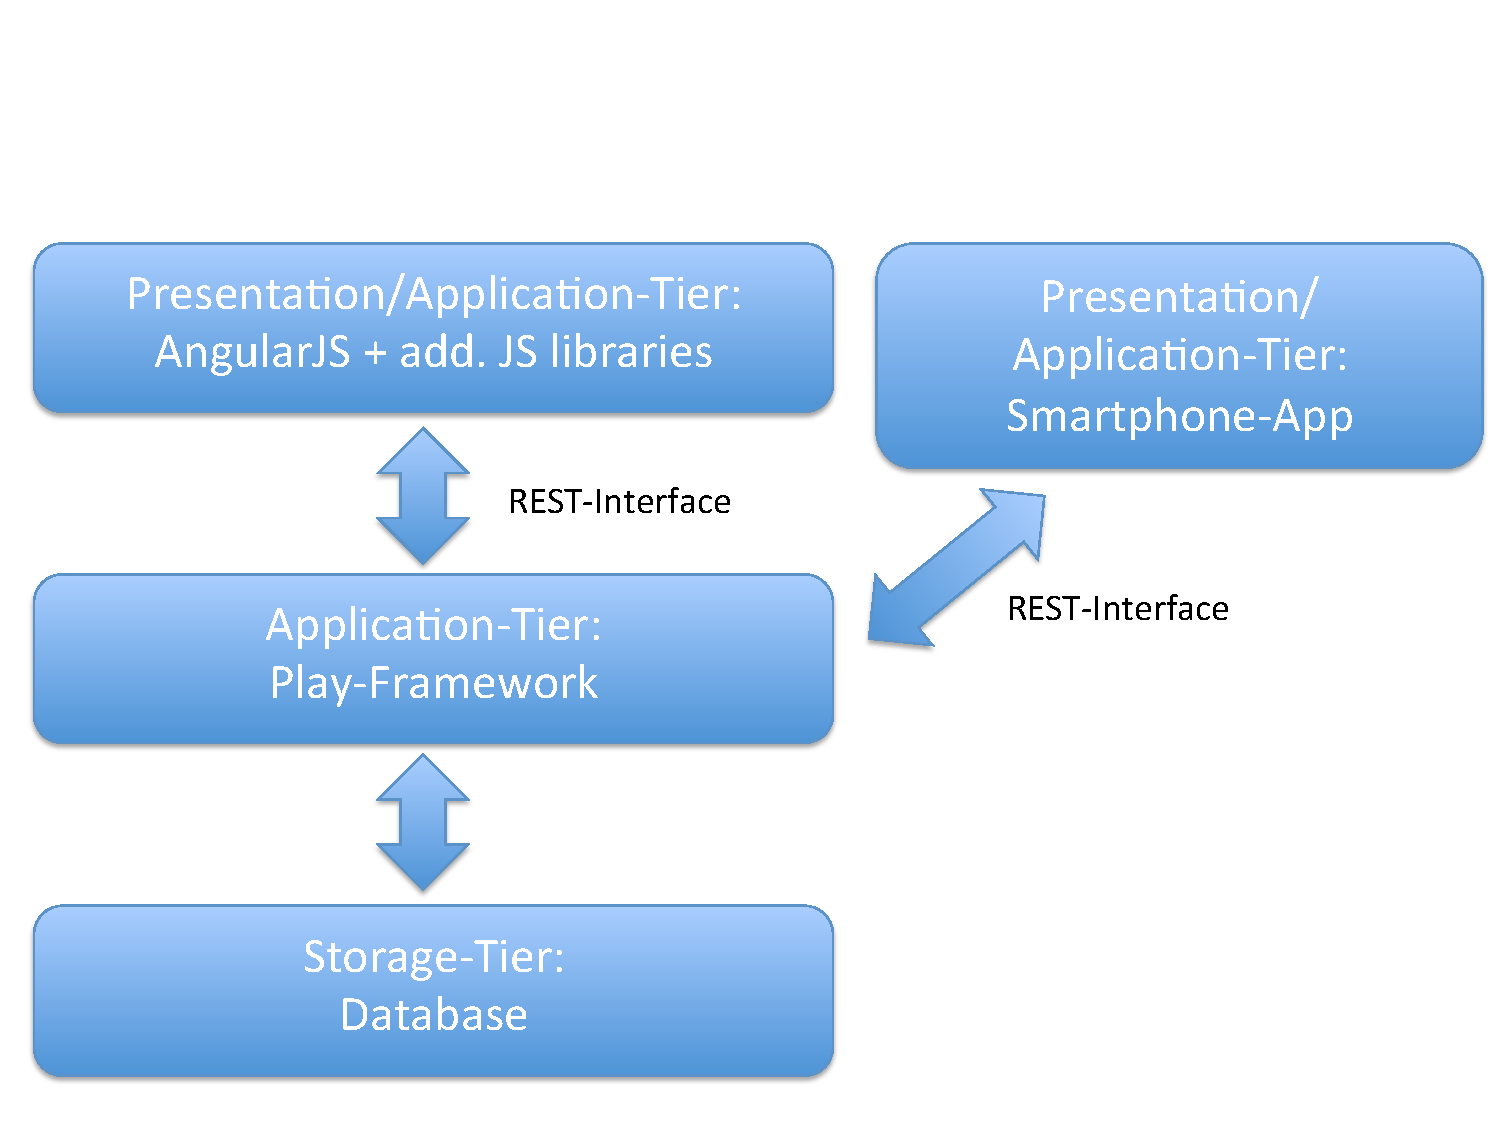
\includegraphics[width=1\textwidth]{gfx/architecture}}
\caption{The general 3-tier architecture of the HiP-application with both presentation tiers (i.e., web frontend and smartphone frontend).}
\label{hip:architecture}
\end{figure}

That said, we will choose a 2-tier 3-layer architecture for the development for the application. This is, according to \cite{Eckerson1995}, a quite common architecture for Client/Server respectively web applications. Within our application, the 3-layer architecture is nice because it enables us to exchange the first tier easily, which is a feature that we will need to support the web-backend and a smartphone front-end. 

The main idea about the architecture is shown in Figure \ref{hip:architecture}. The figure shows also the storage layer, which will be driven by a MongoDB. The data that will be stored in the MongoDB gets prepared by the Play-Framework, which will create the foundation for the application layer on the second tier. Nevertheless, we want to build a fast and application that is able to give instant feedback to the user within the \ac{UI}. Because of that, some parts of the application layer need to be included on the client side within the presentation layer. Because of that, the presentation layer will be much more complex as it is shown in this brief draft since AngularJS, which is used in this layer, relies on a \ac{MVVM} architecture on its own.
However, more detailed decisions about the architecture design are postponed to the \textit{least responsible moment}, as it has been suggested by \cite{Mast2013}.

Now, we have an idea about the general architecture. Nevertheless, we need to take a look at the usage of the different components (e.g., frameworks, libraries and tools) and how they will work together.

\section{Usage of the components}
As we have seen in section \ref{architecture} a lot of application logic will be included in the first layer (i.e., presentation layer). To offer all needed features of the backend in this short time frame, we will need to include a couple of frameworks and libraries. A brief overview about the components and how they work together is shown in Figure \ref{hip:components}. 

 \begin{figure}[th]
\centerline{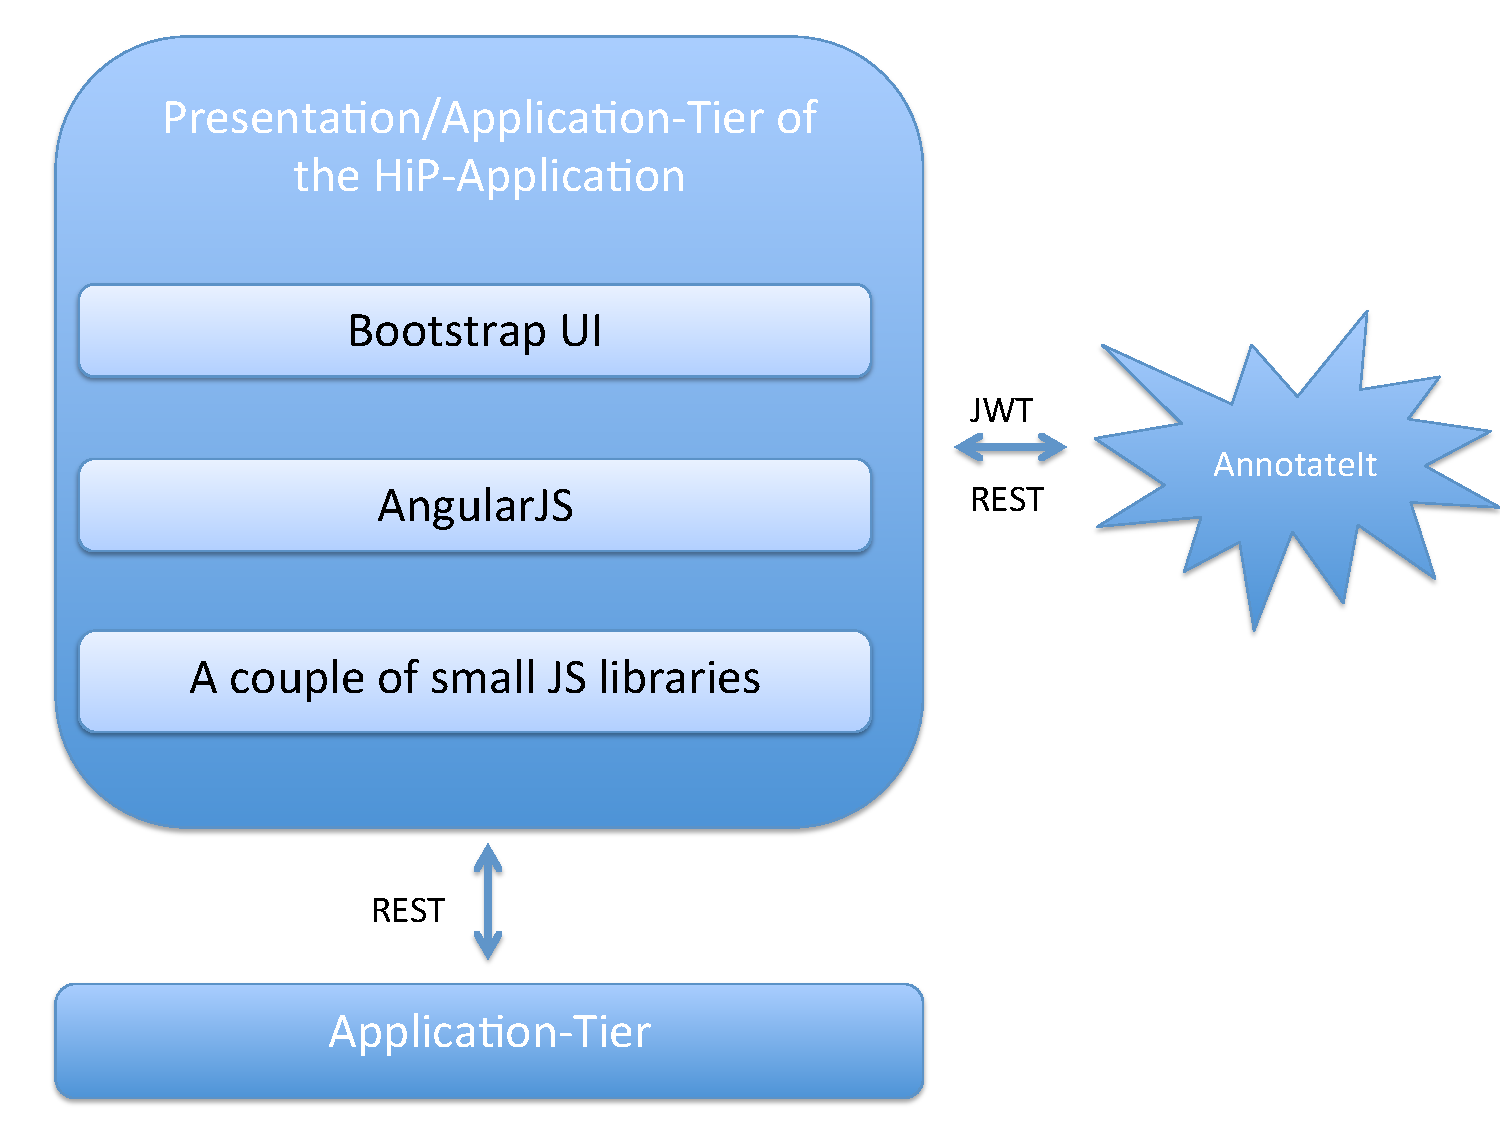
\includegraphics[width=1\textwidth]{gfx/components}}
\caption{The usage of the different components and how they work together}
\label{hip:components}
\end{figure}

The figure shows that the backend system will make use of AngularJS and Bootstrap UI to create the \ac{UI} itself. Furthermore, these two components will be supported by a couple of smaller \ac{JS} libraries for highlighting (i.e., \emph{AnnotatorJS}) or word processing environments (i.e., \emph{textAngular}). To create highlighting with AnnotatorJS that is persistent, we need to send the information via another \ac{REST} interface to storage service.
However, this creates the need for the user of the \ac{HiP} application to register on this backend service, which is not acceptable. This is why the authentication of the user can be pushed from the \ac{HiP} backend to the storage service (i.e., AnnotateIt) with a \ac{JWT}. This \ac{JWT} is a digital claim encoded as a \ac{JSON} object that is digitally signed using a \ac{JWS}. It offers a possibility to represent claims that can be transferred between two parties in a safe way. More details about this authentication process will be shown in chapter \ref{implementation}.

After we have now seen the general architecture and the used frameworks, we will take a look at the different part of the system in more detail.
 
\section{Backend (Web-Server)}
The most important part of the system for this thesis is contained within the backend-web-server. The backend should contain the whole data handling and assessment. The students should be able to add data to the system (e.g., a textual article, graphics, \ac{AR}-data, etc.) and to modify existing data via a \ac{CMS}. These entries get reviewed, for example by the course supervisor and unlocked for the frontend application by an user, who represents the master role. To do this, the backend needs features like annotations and highlighting, which should be private for a specific user. By using this, the supervisor can evaluate the given texts right within the \ac{CMS} and give his final judgement. If the supervisor is not satisfied with the quality of the given text, he should be able to send the document back to the student to get a revised and updated version of the document. If the supervisor is satisfied, he can unlock the information for showing in the frontend application. The whole process is also shown in Figure \ref{workflow_backend}, which can be found in the appendix. The figure shows the complete workflow within the backend system as a flowchart.

The data (i.e., topics, graphics, etc.) should be stored in a way that it can be shown within an \ac{AR}-environment in the smartphone application. Of course, we will need some mechanism to structure the data, for example tags or stored categories. This kind of information (especially tags) are also very important for the described filtering techniques on the client side.

\begin{figure}[ht]
\centerline{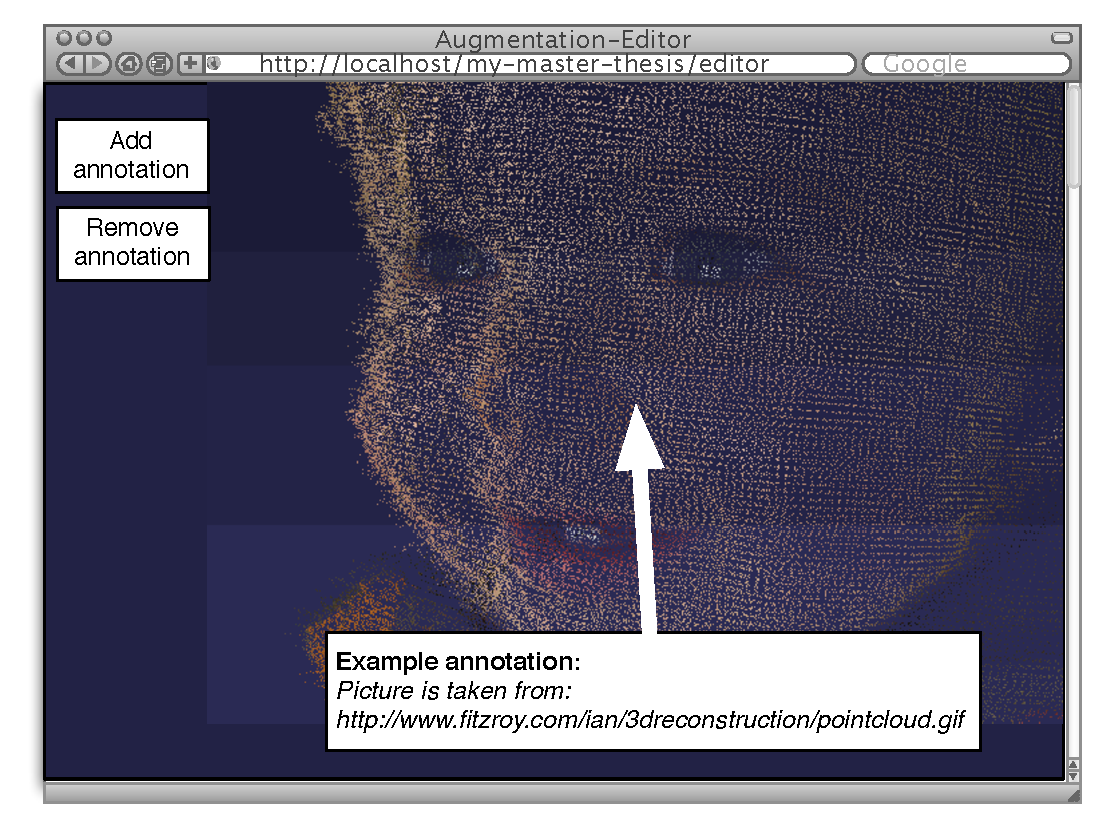
\includegraphics[width=1\textwidth]{gfx/mockup_web_1}}
\caption{A mockup showing the augmentation editor that will be included in the web-application. The editor will be used to edit the point-clouds, which have been added with the help of the smartphone-application}
\label{augmentation_web}
\end{figure}

Furthermore, the backend should include a way to modify the point-clouds of the objects that has been scanned with the smartphone application. It will need features to add annotations directly to these point-clouds to show them afterwards within the \ac{AR}-environment. This editor will be created on the basis of \ac{HTML5} and \ac{WebGL}. A mockup of this site is shown in Figure \ref{augmentation_web}. These annotations should also be assessable and (un-)lockable for the supervisor. 

The following subsections will take a closer look at specific parts of the backend to create a better foundation for the cost estimation at the end of this section. 

\subsection{Input data/content via the \ac{CMS} in the system}
The storage of the data respectively content of the topics and groups will be mainly done by using the MongoDB. For example, a topic will be an object with information like version number, content, etc. 

So, when an user changes something at a topic, the data is changed on the model within the view and send back to the model in the backend. This can be done quite easy with AngularJS because it provides a \ac{HTTP} module that can send \ac{HTTP} requests with a simple call like $http.post(destination,data)$ to update the model with values from the view-model. However, this way of data handling (i.e., modifying on the client side and sending data back as soon as the user hits the \emph{save} button) induces problems if more than one user works at the same time at the same topic. Imagine user $A$ and $B$ start to work at the same topic at the same point in time. Then both download the same content on their client side but if $A$ clicks \emph{save} before $B$, then $B$ will override all changes from $A$. We will prevent this problem by creating a \emph{lock} mechanism on a topic. So, if $A$ works on the topic, $B$ is not able to start editing in the first place. The now induced efficiency problem (i.e., only one user can work at a topic) will be reduced by offering features for creating different text blocks that are autonomously locked. So, $A$ is not locking the topic \emph{S\"udring center} but only a part of it (e.g., \emph{S\"udring center - Introduction}).

Furthermore, the status of the topics should be reflected by constraints (e.g., maximal or minimal characters in the topic) about the topic that get automatically evaluated while the students are working on the topic. 

However, to handle the organization of these topics, we will need to implement groups and their relation to users in the system. So, we will have group documents in the MongoDB, which are linked to the user objects that get returned by the \emph{SecureSocial 2} plugin, which has been explained in section \ref{Play2}.

But including data in the system is not enough for working with topics. We need also ways to offer review features for supervising users. 

\subsection{Manage content as a reviewer}
The reviewer should be able to review the content that gets send in by the students. In this process, he should be able to attach comments to the topic itself and send feedback to the students. This can easily be handled by the \ac{JS} library \emph{AnnotateJS} and will be explained in more detail within chapter \ref{implementation}.

The attachment of information and comments to a complete topic can easily be created by using the chat system and a new chat room, which is exclusively opened for that topic object. 

If the supervisor is satisfied with the given quality, he should be able to mark the topic as 'ready for publish'. On a technical side, this boils down to setting a different flag at the topic object. So, the needed time for this feature should be low.

\subsection{Including a 3D-Tooling system for point-clouds (WebGL)}
The augmentation editor will be needed to edit the objects (i.e., point clouds) that have been scanned with a smartphone by a student. 
\todo{mehr}
The editor should be able to show the stored point-clouds and attach objets (for example images) to it. These images can, for example, contain annotations and/or further information. Figure \ref{augmentation_web} shows a mockup of such a system. 
\todo{technical details}

\subsection{Cost estimation of the backend}
\label{backendEstimation}
Now, as we have seen the major ideas about the backend, we will try to create a rough cost-estimation about the backend. The story points have been explained in section \ref{storyPoints} and should represent 6 hours per point. This way, we get only a rough estimation. Nonetheless, this rough estimation should be sufficient to get an idea about the needed time. However, note that some parts of the system could be subject for change because we are using an agile approach and some new requirements may come up within the development process.

 \begin{table}[h]
\scriptsize
 \caption{A brief cost-estimation about the backend}
 \begin{tabular}{lll}
	\toprule
  Name & Description & Story points \\ 
\cmidrule(rl){1-1}\cmidrule(rl){2-2}\cmidrule(rl){3-3}
	Create login system		&	Login needed for right/role management			&	2 \\	
	Create language system	&	The system should be able to handle multiple languages&	2 \\	
	Create chat system		&	Chats are needed for (group-) communication between &	1 \\	
		 				&	users of the system (e.g., in topics)					&	 \\	
	Create message system &	Messages are needed for direct communication between&	1 \\
	 					&	users of the system 							&	 \\		
  	Create group system 	& 	Groups will be needed for organization of students 	& 	2 \\
  	Create topic system 	& 	Topics will be the main objects, which can be changed  	& 	10 \\
  	 					& 	by students  								 	&	   \\
	Create constraint system  &	Constrains should be created by supervisors and 		&	4 \\
						&	are automatically evaluated						&	   \\	
  	Create annotation system & 	Content of topics should be able to be annotated  		& 	3 \\
  	 					& 	by students  (e.g, highlighted)						&	   \\
  	Create \ac{AR} - editing  & 	The 3D objects should be editable by the students 	& 	4 \\
  	 system				& 												&	   \\
	Add tooltips			&	The main features should be explained with tooltips	&	1 \\
	Media upload			&	The user should be able to upload multiple media formats	&	1 \\
	  	 				& 	like pictures, 3D objects, etc.						&	   \\
	Create version system	&	One should be able to restore/compare different versions &	4 \\	
		  	 			& 	of a topic										&	   \\
				  	 	& 												& $\sum$ $35$   \\
	\bottomrule
 \end{tabular}
 \label{tab:costBackend}
 \end{table} 

Table \ref{tab:costBackend} shows that the backend system needs a lot of typical \ac{CMS} functions, which sum up to $35$ story points. So, the backend system should cost about $210$ hours to create a prototypical but running system. 

\section{Frontend (App)}
\begin{figure}[th]
\centerline{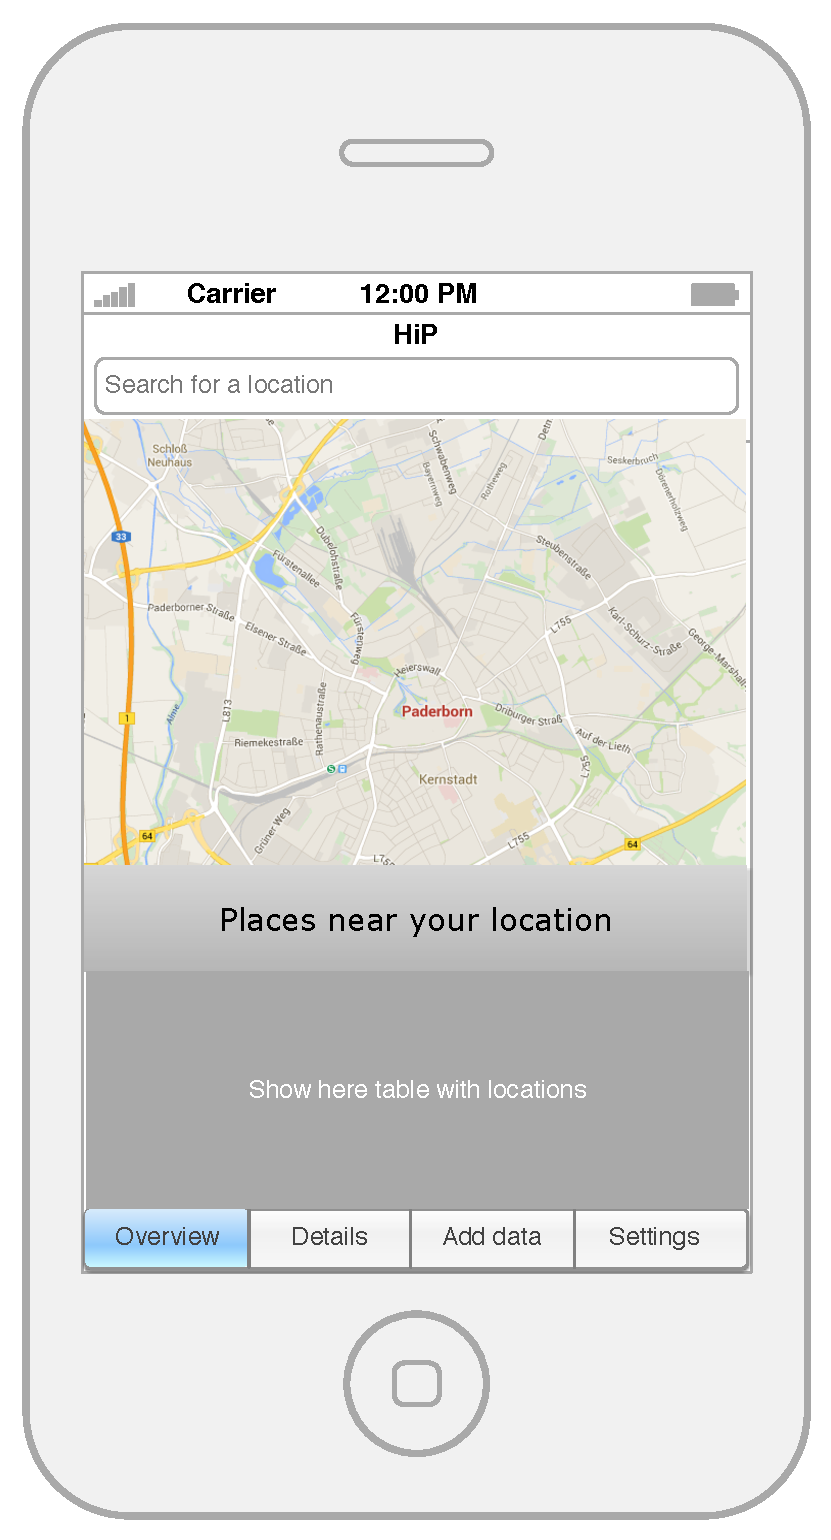
\includegraphics[width=0.5\textwidth]{gfx/mockup_app_1}}
\caption{A mockup showing the main page of the frontend application showing a map of paderborn and a general overview about the UI-elements}
\label{app1}
\end{figure}

The smartphone application is the part of the system that gets shipped to the end-user (respectively downloaded via an App-Store like Google-Play). The user can use the app to find interesting places respectively objects in Paderborn and is able to start a navigation to the place/object easily. Furthermore, the user can get an overview about all places in Paderborn by activating a map that shows all entries within the system. A mockup of this view is shown in Figure \ref{app1}. Of course, the user will be able to set up specific filters like 'show only art', 'show only historic buildings' or 'use simplified language' to adapt the system to his own experiences and educational qualifications. Moreover, if the university courses would add information over years, the system will need filtering features like this to handle the complexity of the data.

After an user has reached an interesting place, he can use the details tab to switch into the \ac{AR}-mode. With this view, the user can use the smartphone-camera to embed information, which has been added via the backend, right into the picture of the object. An mockup of this view is shown in Figure \ref{app2}. 
To create a feasible input for the \ac{AR} system, the user should be able to scan objects in 3D directly with his smartphone and send the data (i.e., a point-cloud of the scanned object), back to the web-server.  Afterwards, the user can add annotations to the point-cloud via the web-backend of the system. 

In the following, we will focus on the planning and cost estimations off the frontend applications because our actual prototypical implementation contains only the backend system.  However, code examples (for Android) and ideas will be included within the draft. 

\begin{figure}[th]
	\centerline{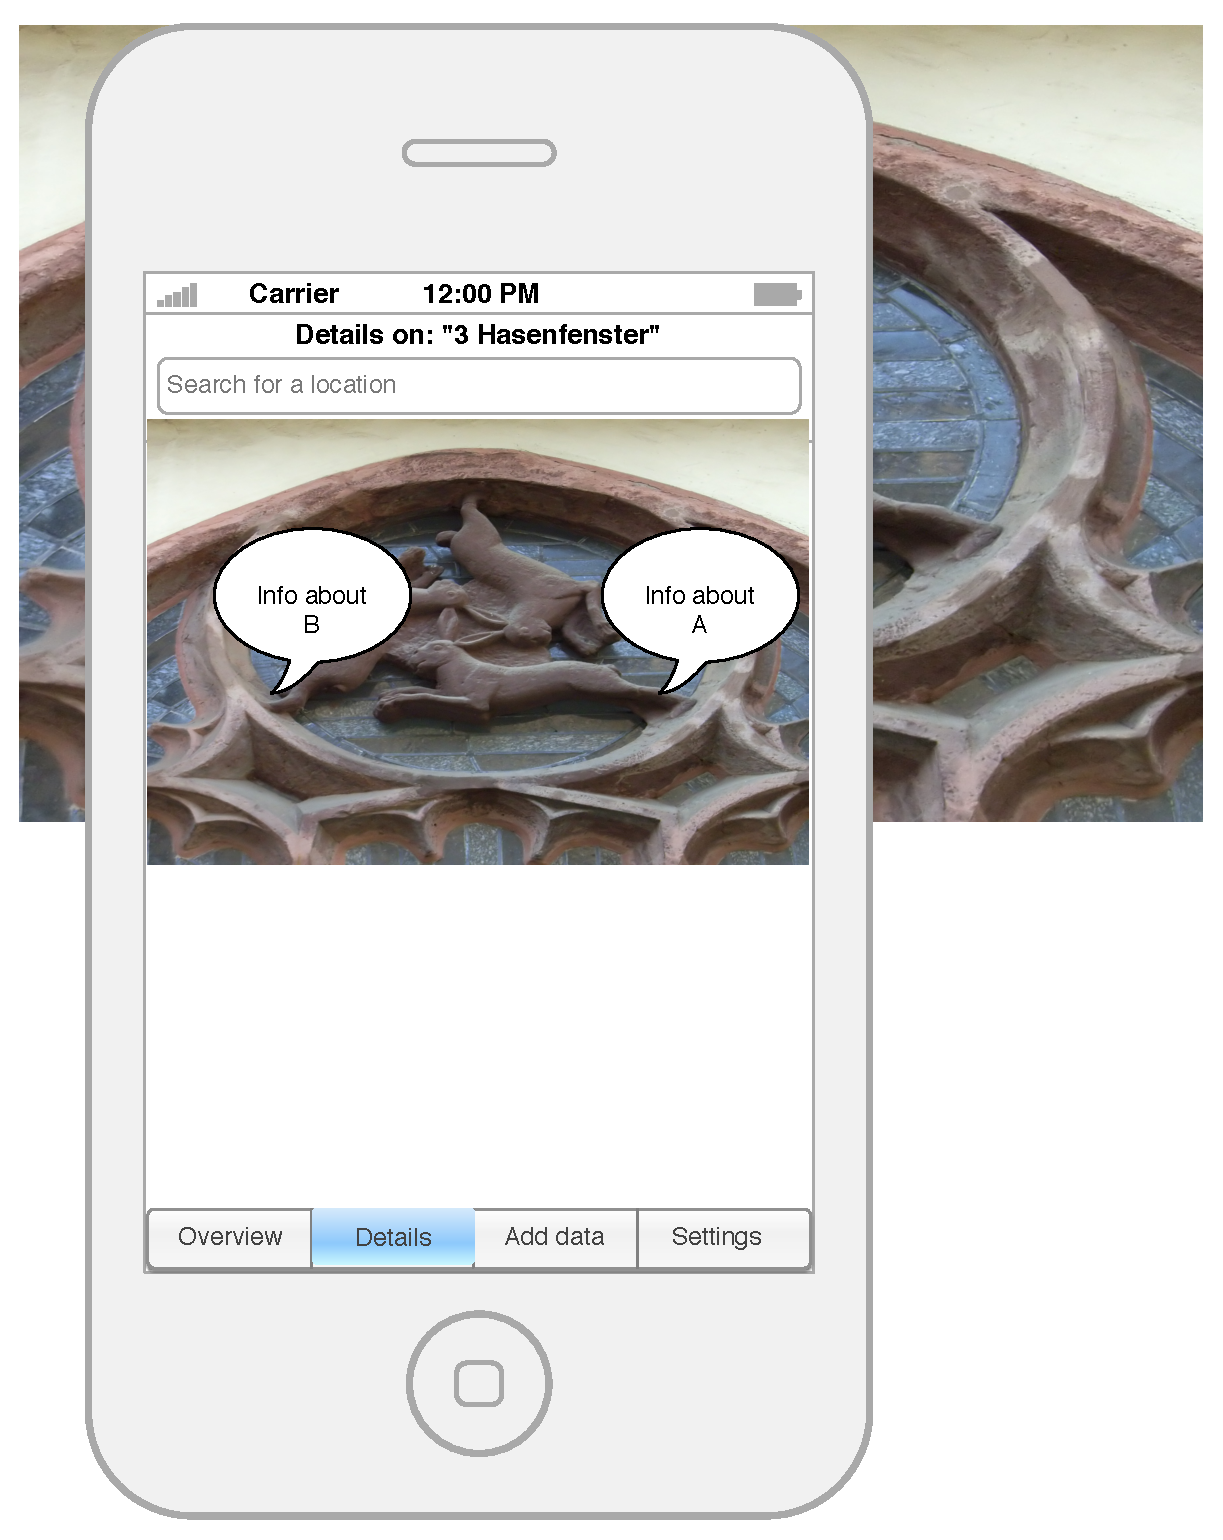
\includegraphics[width=0.7\textwidth]{gfx/mockup_app_2}}
	\caption{A mockup showing the details page of the "Dreihasenfenster" while the camera of the smartphone is pointing to the window itself}
	\label{app2}
\end{figure}			
  
\subsection{Input data into the system (scan objects and annotate them)} 
With the Junaio eco-system of the company Metaio it is quite easy to scan objects and store them as point clouds that can be used to track the object with Junaio. The scanning process itself is done by the \emph{Metaio Toolbox}. A screenshot of the \emph{Metaio Toolbox} is shown in Figure \ref{MetToolbox}. When an object gets scanned with the Toolbox, the file is stored on the smartphone's filesystem and can be shared by using email attachments \todo{more}.

\begin{figure}[th]
	\centerline{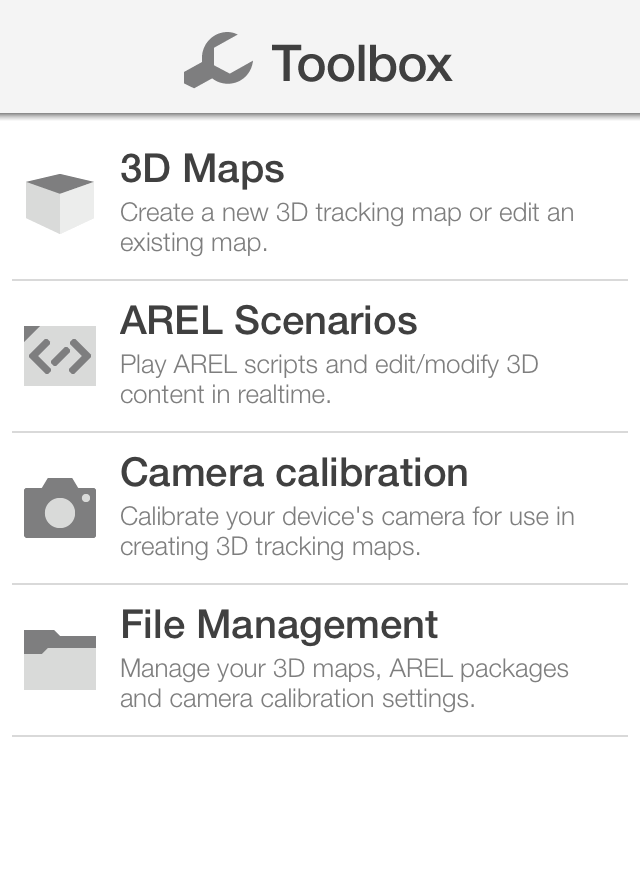
\includegraphics[width=0.5\textwidth]{gfx/toolbox.png}}
	\caption{The main menu of the \emph{Metaio Toolbox} showing the main features of the app.}
	\label{MetToolbox}
\end{figure}	

\subsubsection{Data format for \ac{AR} files}
The scanned objects are saved within the \emph{3dmap} and \emph{creator3dmap} format. Both files are essentially ZIP files that contain metadata, pictures and binary data for the point-clouds. The original idea within this thesis was to use these files to render the point-clouds in the backend and offer features for manipulation. However, because we would need the file specification to be able to read the binary data contained in the ZIP files, we asked for such a specification at the company Metaio. Sadly, we never received an answer. 

Thus, this part of the thesis is postponed and left open for the Project Group.

\subsection{Show close "interesting places" within a map} 
In the end, every topic will contain \ac{GPS} coordinates for exhibits and locations, which has been added by students. We can make use of this information to get a location specific map and navigation features on the smartphone. 

\lstset{language=Java,
basicstyle=\small,
showspaces=false,
showstringspaces=false,   
tabsize=2,
backgroundcolor=\color{grey}}
\begin{lstlisting}[numbers=left,caption={Example for using the GPS coordinates within an Android application},label=Android:GPS,frame=tlbr,breaklines]
import com.google.android.gms.maps.*;
import com.google.android.gms.maps.model.*;
import android.app.Activity;
import android.os.Bundle;

public class MapPane extends Activity implements OnMapReadyCallback {

    @Override
    protected void onCreate(Bundle savedInstanceState) {
	      /* some initialization data */
    }

    @Override
    public void onMapReady(GoogleMap map) {
        LatLng paderbornDom = new LatLng(51.718889, 8.755278);

        map.setMyLocationEnabled(true);
        map.moveCamera(CameraUpdateFactory.newLatLngZoom(paderbornDom, 13));

        map.addMarker(new MarkerOptions()
                .title("Paderborner Dom")
                .snippet("The cathedral of the Catholic Archdiocese of Paderborn")
                .position(paderbornDom));
    }
}
\end{lstlisting}

The usage of the \ac{GPS} information is quite easy within Android because we can make use of the \emph{Google Maps API}. As Listing \ref{Android:GPS} shows, we can directly manipulate the Google Maps view by using the $LatLng$ object. Line 18 shows the movement of the camera (i.e., the excerpt of the map) and line 20 the creation of a marker on the map. 

\subsection{Navigation to "interesting places"}
An easy way to create a navigation feature would be the usage of the Google directions service (\cite{GoogleNavi}). However, this service runs not natively on Android, so we would need a wrapper to access the \ac{HTML} and \ac{JS} based source code in our Android application. 

\lstset{language=Java,
basicstyle=\small,
showspaces=false,
showstringspaces=false,   
tabsize=2,
backgroundcolor=\color{grey}}
\begin{lstlisting}[numbers=left,caption={Example for construction of the DirectionsRequest JSON object that is needed to use the directions service},label=Android:dirService,frame=tlbr,breaklines]
{
  origin: LatLng | String,
  destination: LatLng | String,
  travelMode: TravelMode,
  transitOptions: TransitOptions,
  unitSystem: UnitSystem,
  waypoints[]: DirectionsWaypoint,
  optimizeWaypoints: Boolean,
  provideRouteAlternatives: Boolean,
  avoidHighways: Boolean,
  avoidTolls: Boolean
  region: String
}
\end{lstlisting}

After doing that, we can access the direction service by posting a \ac{JSON} object to the Google service and use the returned data to render the navigation path within our application. The construction of such a \ac{JSON} object is shown in Listing \ref{Android:dirService}. 

As we can see, this object include information like the position of the navigation origin, the position of the destination and specific travel options (e.g., using train, car, etc.). After we have send this object, we need to render the returned data. This is, for example, possible by drawing lines on the map using the $google.maps.Polyline$ class. This is shown in Listing \ref{Android:polyline}.

\lstset{language=Java,
basicstyle=\small,
showspaces=false,
showstringspaces=false,   
tabsize=2,
backgroundcolor=\color{grey}}
\begin{lstlisting}[numbers=left,caption={Example for writing a poly line on the google map},label=Android:polyline,frame=tlbr,breaklines]
function initialize() {
  var mapOptions = {
         /* positioning of the map */
  };

  var map = new google.maps.Map(document.getElementById('map-canvas'),
      mapOptions);

   /* array with the coordinates */
  var flightPlanCoordinates = [
    new google.maps.LatLng(37.772323, -122.214897),
    [...],
  ];
  var flightPath = new google.maps.Polyline({
    path: flightPlanCoordinates,
    [...] // options for the rendering of the polyline
    strokeColor: '#FF0000'
  });

  flightPath.setMap(map);
}

google.maps.event.addDomListener(window, 'load', initialize);
\end{lstlisting}

As we can see in Listing \ref{Android:polyline}, we can directly draw on the map, which is really fast. The listing shows the code in Javascript. The flightPath object is directly created as a Polyline object with the given coordinates. After that, it can directly be placed on the map. Although the shown code is \ac{JS}, the Polyline class can, however, be accessed natively with the Android SDK (\cite{GooglePolylineNative}). Obviously, the simplicity of the usage of the Google Maps API is a good foundation for more complex functionality, like the treasure hunt respectively geocaching functionality, which has been expressed within the first requirements meeting. One just needs to create an array of $LatLng$ objects from the locations that should be used as waypoints, the remaining work is done from the Google directions service.  

Another, more complex but more powerful, approach would be to fork the \ac{OsmAnd} project and use the code as a basis for the HiP-Navigation feature. \ac{OsmAnd} is a map and navigation application that uses the \ac{OSM} data. The application offers routing with optical and voice guidance and navigation for car, bike, and pedestrian (\cite{osmand}). Furthermore, all main functionalities can be used online and offline, which is nice, because we can directly include the needed maps for the area of paderborn. This would reduce the load on the internet connection of the mobile device (i.e., smartphone). Another great feature of \ac{OsmAnd} is that it is capable of using different map overlays. An example for such an overlay is one for touring features. These functions could be modified within the HiP-Application to render different city plans (e.g., from different epochs). Last but not least, \ac{OsmAnd} supports intermediate points on your route, which can be modified for the treasure hunt functionality.

However, by using \ac{GPS} we are only able to creating a good location awareness for outdoor situations. As soon as the user of the smartphone enters building, we need to think about other ways to get a precise estimation about the position of the user. The smartphone application could include this by using iBeacons. 
An iBeacon is a new approach for creating very precise location estimations that has been developed by Apple. Technically, \ac{BLE} is used to connect to a device that supports the iBeacon technology within a region around the device (i.e., the object that has the iBeacon device attached). This allows a smartphone to determine whether it has entered or left the region and to create an estimation about the proximity to the beacon (\cite{Apple:2014aa}). Natively, only iOS since version 7.0 offers support for the usage of iBeacon.

However, there exist a couple of libraries on the Android platform that offer solutions for creating iBeacon functionality for Android. Two of these libraries are created by Radius Networks and Sensorberg. Sensorberg's solution was for example used to create the iBeacon based indoor navigation at the Cebit 2014 (\cite{Kaufmann:2014aa}). However, Sensorberg focuses on the distribution of own hardware in combination with its library. So, the library of Radius Networks called \emph{Android Beacon Library}, which offers mainly its library licensed under the Apache License Version 2.0, is more interesting for our project. The library allows Android devices to use beacons in a similar way like iOS devices. This means, every app using this library on the Android smartphone can request to get notifications when the smartphone reaches a close range to a beacon respectively leaves it (\cite{RadiusNetworks:2015aa}). 

The usage of the library is very easy and fast. One only needs to derive a new class from a class that is included within the library and overwrite a couple of methods. For example, by a simple overwrite of the method \emph{didEnterRegion(Region region)} one can handle the reaction of the smartphone application when a new iBeacon has been found (\cite{RadiusNetworks:2015ab}).   

But, as we have stated before, forking this project to create the \ac{HiP}-navigation application results in much more work but we end up with a complete navigation application with every common function. 

\subsection{Fetching topics and PDF export}
As soon as an user arrives at a specific location, he is able to gather data about the object and collect the information he wants. On a technical level, this is a simple \ac{HTTP} GET request to our backend to download the information.

\lstset{language=Java,
basicstyle=\small,
showspaces=false,
showstringspaces=false,   
tabsize=2,
backgroundcolor=\color{grey}}
\begin{lstlisting}[numbers=left,caption={Creation and usage of an Android HTTP client},label=Android:HTTP,frame=tlbr,breaklines]
/* init variables */
[...]

/* create HTTP client */
HttpClient httpclient = new DefaultHttpClient();

HttpGet request = new HttpGet();
URI url = new URI("http://yourHipServer/topics/uIDOfATopic");
request.setURI(url);

/* send request and get response*/
HttpResponse response = httpclient.execute(request);

/* read response */
in = new BufferedReader(new InputStreamReader(response.getEntity().getContent()));
String line = in.readLine();
textv.append(" First line: " + line);
\end{lstlisting}

As Listing \ref{Android:HTTP} shows, it is only a matter of a couple of lines to create a \ac{HTTP} client for Android. Line $5$ shows the creation of a $HttpClient$ object, which is used in line $12$ to send the GET request.

Another important thing is the \ac{PDF} export functionality of the data that we have just downloaded from our backend server.
Because there is no out-of-the-box way on Android to create \ac{PDF} documents, we need to make use of an external library. One choice for such a library is $iText$. This is a \ac{PDF} library for Android that offers features to create, adapt and maintain \ac{PDF} document (\cite{itext2015}).
With this library, it is quite easy to export the downloaded data to a \ac{PDF} file because we can directly create chapters and section with content within our \ac{PDF} file. For doing this, we can make use of classes like $chapter$, $Paragraph$ and similar environments (\cite{pdfCreation}). The creation of a new paragraph could for example look like:

\verb|myCategory.add(new Paragraph("This is a very important message"));|  

All in all, \ac{PDF} export can be included fast and easy within the smartphone application.

\subsection{Rendering AR-data with Junaio}
The rendering of the \ac{AR} data is another very important part of the \ac{HiP} frontend. As it has been explained in section \ref{AREL}, we need to create a static content definition, a \ac{HTML5} layer and the application logic. While the application logic can be general for the whole application, we need to generate the static content definition and the \ac{HTML5} layer for every topic because the shown objects are changed, as soon as we change a topic.
\todo{more}

\subsection{Cost estimation of the frontend}	
Now, after we have seen the technical details about the different parts of the frontend, we can create our cost estimation. One problem is that the cost estimation of the frontend is quite complex and depends heavily on the choice of the basis for the navigation feature. Thus, we assume in the following that we use the \ac{OsmAnd} project as the basis for the \ac{HiP}-navigation features. Like in section \ref{backendEstimation}, one story point should represent 6 hours.

 \begin{table}[th]
\scriptsize
 \caption{A brief cost-estimation about the frontend}
 \begin{tabular}{lll}
	\toprule
  	Name & Description & Story points \\ 
	\cmidrule(rl){1-1}\cmidrule(rl){2-2}\cmidrule(rl){3-3}
	Create running prototype		&	We need to set up a running Android application that can be			&	5 \\	
							& 	 used as a starting point for the \ac{HiP} frontend					& 	\\
	Showing locations on map	&	The exhibits and locations should be shown on the map			&	3 \\	
	Download data and PDF	 	&	More information should be downloaded as soon as the user		&	4 \\	
	export					& 	arrives at the position. After that, he is able to export the data		&	\\
							& 	to a \ac{PDF} document										& 	\\
	Include treasure hunts, etc.	&	The user should be able to join treasure hunts within Paderborn		&	2 \\	
	Include the Junaio framework	&	The user should be able to render AR-information, as soon as he		&	6 \\			
							&	arrives at a specific position									&	\\
	Include iBeacon support		&	The user should be able to get information about iBeacons on its		&	3 \\			
							&	location													&	\\
	Fork and understand \ac{OsmAnd}	&	We need to find the important parts of \ac{OsmAnd} for the \ac{HiP}	&	6 \\
							&	application. To find out, what we need to include and how 			&	\\
							&	this is possible												& \\
	Include needed parts of \ac{OsmAnd}	&	Include the needed parts of \ac{OsmAnd} in the \ac{HiP} application	&	8 \\	
					  	 	& 												& $\sum$ $37$   \\			
	\bottomrule
 \end{tabular}
 \label{tab:costFrontend}
 \end{table} 

Table \ref{tab:costFrontend} shows the minimal features of the smartphone frontend, which sum up to $34$ story points. So, the frontend system should cost about $222$ hours to create a prototypical but running system. 
